%%%%%%%%%%%%%%%%%%%%%%%%%%%%%%%%%%%%%%%%%%%%%%%%%%%%%%%%%%%%%%%%%%%%%%%%%%%%%%%%%%%%%%%%%%%%%%%%%%%%%%%%%%%%%%%%%%%%%%%%%
% master.tex                                                                                                            %
% This file specifies things like general formatting, font sizes, page numbering, etc.                                  %
% It also tells the compiler where to look for the .tex files for the title page, abstract, chapters, bibliography, etc %
% See the README file for compilation information                                                                       %
% Template written by John Groh                                                                                         %
%%%%%%%%%%%%%%%%%%%%%%%%%%%%%%%%%%%%%%%%%%%%%%%%%%%%%%%%%%%%%%%%%%%%%%%%%%%%%%%%%%%%%%%%%%%%%%%%%%%%%%%%%%%%%%%%%%%%%%%%% 

\documentclass[12pt,oneside]{book}

\usepackage{amsmath}                 % math stuff
\usepackage{amssymb}                 % more math stuff
\usepackage{graphicx}                % including figures
\usepackage[lofdepth]{subfig}        % subfigures
\usepackage[left=1.0in,right=1.0in,%
  top=1.0in,bottom=1.0in]{geometry}  % margin control
\usepackage[toc,page]{appendix}      % appendix stuff
\usepackage{times}                   % Times New Roman font
\usepackage{color}                   % colored text
\usepackage{float}                   % allows for [H] option with figure placing
\usepackage[square, numbers]{natbib} % nicer citing
\usepackage{indentfirst}             % indents first paragraph of every section
\usepackage{setspace}                % manual line spacing control
\usepackage{fancyhdr}                % these 5 lines are for header/footer:
\fancypagestyle{plain}{
\fancyhead[R]{\thepage}\fancyhead[L]{}\fancyfoot[C]{}
\renewcommand{\headrulewidth}{0pt}}
\pagestyle{plain}
\setlength{\headheight}{15pt}
\usepackage{titlesec}                % these 4 lines are for formatting chapter titles:
\titleformat{\chapter}[display]
{\normalfont\Huge\bfseries\centering}
{\vspace{8ex}\chaptertitlename\ \thechapter}{20pt}{\Huge}
\renewcommand{\bibname}{References}

\usepackage{algorithm}
\usepackage{algorithmic}
\usepackage{booktabs}
\usepackage{graphicx}
\usepackage{multirow}
\usepackage[intoc]{nomencl}
\makenomenclature


\begin{document}
% Include all the front matter.  Each command is independent of the others, so commenting out a line will cause
% it to not be included in the compilation
\frontmatter
%%%%%%%%%%%%%%%%%%%%%%%%%%%%%%%%%%%%%%%%%%%%%%%%%%%%%%%%%%%%%%%%%
% titlepage.tex                                                 %
% This file gives the formatting and contents of the title page %
%%%%%%%%%%%%%%%%%%%%%%%%%%%%%%%%%%%%%%%%%%%%%%%%%%%%%%%%%%%%%%%%%

\begin{titlepage}
\center % center everything on the page

\vspace*{1.0cm}
THE PENNSYLVANIA STATE UNIVERSITY\\
SCHREYER HONORS COLLEGE\\[1.0cm]
DEPARTMENT OF AEROSPACE ENGINEERING\\[1.0cm]
Parallelized Particle Swarm Optimization for Minimum-Time Satellite Orientation Maneuvers \\[1.0cm]
Sean Rich\\
Spring 2020\\[1.0cm]
A thesis\\
submitted in partial fulfillment\\
of the requirements\\
for a baccalaureate degree\\
in Aerospace Engineering\\
with honors in Aerospace Engineering\\[1.0cm]

Reviewed and approved* by the following:\\[0.5cm]
Robert G. Melton\\
Professor of Aerospace Engineering\\
Director of Undergraduate Studies\\
Thesis Supervisor and Honors Advisor\\[0.5cm]

Amy R. Pritchett\\
Professor and Head of the Department of Aerospace Engineering\\
Faculty Reader\\[0.5cm]

*Electronic approvals are on file in the Schreyer Honors College.

\end{titlepage}
 % see titlepage.tex
%%%%%%%%%%%%%%%%%%%%%%%%%%%%%%%%%%%%%%%%%%%%%%%%%%%%%%%%%%%%%%
% abstract.tex                                               %
% This file formats and includes the content of the abstract %
%%%%%%%%%%%%%%%%%%%%%%%%%%%%%%%%%%%%%%%%%%%%%%%%%%%%%%%%%%%%%%

\cleardoublepage
\thispagestyle{empty} % no page numbers on this page

\chapter*{Abstract} % make this a \chapter* to not include it in the table of contents

\noindent Particle swarm optimization has developed as a popular method of solution 
discovery for many numerical problems. The finite thrust transfer problem employs
this metaheuristic algorithm for trajectory optimization.  This method is computationally expensive and requires
numerous runs to confidently discover a quasi-optimal solution. These major bottlenecks - execution time and 
a low probability of optimal solution convergence - make real-time, on-board calculations utilizing this algorithm 
impractical. \newline

\noindent The research presented within this thesis studies two methods to significantly improve each of these bottlenecks.
This thesis develops results that show increased algorithm performance of well over an order of magnitude, and demonstrably
improves the average solution discovered. In employing these two methods in concert, this
research suggests the potential feasibility of real-time particle swarm optimization techniques.\newline

\cleardoublepage
 % etc.
%%%%%%%%%%%%%%%%%%%%%%%%%%%%%%%%%%%%%%%%%%%%%%%%%%%%%%%%%%%%%%%%%%%%%%%%%%%%%%%%%%%%%%%%%%%%%%%%%%
% table_of_contents.tex                                                                          %
% This file formats and creates the table of content. You shouldn't need to change anything here %
%%%%%%%%%%%%%%%%%%%%%%%%%%%%%%%%%%%%%%%%%%%%%%%%%%%%%%%%%%%%%%%%%%%%%%%%%%%%%%%%%%%%%%%%%%%%%%%%%%

\renewcommand{\contentsname}{Table of Contents} % changes the title to appease Schreyer
\tableofcontents
\cleardoublepage

%%%%%%%%%%%%%%%%%%%%%%%%%%%%%%%%%%%%%%%%%%%%%%%%%%%%%%%%%%%%%%%%%%%%%%%%%%%%%%%%%%%%%%%%%%%%%%%%%%%%%%%%%%%%%%%%%%%
% list_of_figures.tex                                                                                             %
% This file includes the instructions for adding the list of figures. You shouldn't need to make any changes here %
%%%%%%%%%%%%%%%%%%%%%%%%%%%%%%%%%%%%%%%%%%%%%%%%%%%%%%%%%%%%%%%%%%%%%%%%%%%%%%%%%%%%%%%%%%%%%%%%%%%%%%%%%%%%%%%%%%%

\addcontentsline{toc}{chapter}{\listfigurename}
\listoffigures

%%%%%%%%%%%%%%%%%%%%%%%%%%%%%%%%%%%%%%%%%%%%%%%%%%%%%%%%%%%%%%%%%%%%%%%%%%%%%%%%%%%%%%%%%%%%%%%%%%%%%%%%%%%%%%
% list_of_tables.tex                                                                                         %
% This file gives instructions for including the list of tables. You shouldn't need to make any changes here %
%%%%%%%%%%%%%%%%%%%%%%%%%%%%%%%%%%%%%%%%%%%%%%%%%%%%%%%%%%%%%%%%%%%%%%%%%%%%%%%%%%%%%%%%%%%%%%%%%%%%%%%%%%%%%%

\addcontentsline{toc}{chapter}{\listtablename}
\listoftables

%%%%%%%%%%%%%%%%%%%%%%%%%%%%%%%%%%%%%%%%%%%%%%%%%%%%%%%%%%%%%%%%%%%%%%%%%%%%%%
% acknowledgements.tex                                                       %
% This file formats and includes the content of the acknowledgements section %
%%%%%%%%%%%%%%%%%%%%%%%%%%%%%%%%%%%%%%%%%%%%%%%%%%%%%%%%%%%%%%%%%%%%%%%%%%%%%%

\cleardoublepage
\thispagestyle{empty}

\chapter{Acknowledgements}
\noindent The creation of this thesis involved significant support from many
throughout this journey. While lots have undoubtedly helped me grow
both academically and personally, there are a few I would like to express my 
sincere gratitude to. \newline

\noindent First, to my thesis advisor, Dr. Melton. His subject matter expertise is obvious, yet, 
perhaps more importantly, so is his passion for teaching others. Whether through classes or this research,
Dr. Melton consistently strives for the best for his students. Dr. Melton has been a beacon in my academic 
and personal undergraduate experience and I cannot thank him enough. \newline

\noindent Second, to my mother Brenda and sister Lindsey. You two have unwaveringly supported me 
in every one of my undertakings for as long as I can remember. 
You have pushed me, loved me, and helped shape me into the person I am today.
You two are my rocks. I love you both endlessly.\newline

\noindent Lastly, to my friends. You make every day enjoyable and have shown me what happiness looks and
feels like. I am so thankful to have you by my side every day; you know I will always be by yours.
\cleardoublepage

\nomenclature{$\Delta t_{co}$}{Coasting time interval}
\nomenclature{$\Delta t_2$}{Thrust arc 2 duration}
\nomenclature{$\Delta t_1$}{Thrust arc 2 duration}
\nomenclature{$J$}{Cost function value}
\nomenclature{$t_0$}{Initial time}
\nomenclature{$v_\theta$}{Transverse velocity component}
\nomenclature{$T$}{Spacecraft thrust}
\nomenclature{$t_f$}{Final time}
\nomenclature{$r$}{Spacecraft position}
\nomenclature{$c$}{Effective exhaust velocity}
\nomenclature{$\delta$}{Thrust pointing angle}
\nomenclature{$\mu_B$}{Gravitational parameter}
\nomenclature{$\xi$}{Spacecraft angular displacement from the $x$ axis}
\nomenclature{$m$}{Spacecraft mass}
\nomenclature{$R_1$}{Initial orbit radius}
\nomenclature{$R_2$}{Final orbit radius}
\nomenclature{$e$}{Eccentricity}
\nomenclature{$m_f$}{Final spacecraft mass}
\nomenclature{$m_0$}{Initial spacecraft mass}
\nomenclature{$f$}{True anamoly}
\nomenclature{$\Delta E$}{Eccentric anamoly change during $t_{co}$}
\nomenclature{$\alpha_k$}{Penalty coefficients}
\nomenclature{$d_k$}{Error terms}
\nomenclature{$\zeta_0$, $\zeta_1$, $\zeta_2$, $\zeta_3$}{Thrust pointing angle coefficients for thrust arc 1}
\nomenclature{$\nu_0$, $\nu_1$, $\nu_2$, $\nu_3$}{Thrust pointing angle coefficients for thrust arc 2}
\nomenclature{$J_{avg}$}{Average global best cost function value over multiple algorithm executions}
\nomenclature{$\delta_J$}{Average $J$ change over previous $n_{iter}$}
\nomenclature{$\Delta J_\%$}{Percent change of $J_{avg}$ for rehydration executions relative to non-rehydration  }
\nomenclature{$n_{iter}$}{Iterations to average $\delta_j$ over}
\nomenclature{$a$}{semi-major axis}
\nomenclature{DU}{One canonical distance unit}
\nomenclature{TU}{One canonical time unit}
\nomenclature{$n_{su}$}{$\frac{\text{MATLAB execution time}}{\text{C++ execution time}}$ }
\nomenclature{$n_{su\%}$}{Percent speed-up relative to MATLAB}
\nomenclature{$n_{sust\%}$}{Percent speed-up relative to C++ single threaded}
\nomenclature{$h$}{Integration step size }

\printnomenclature


% same for the mainmatter
\mainmatter
%%%%%%%%%%%%%%%%%%%%%%%%%%%%%%%%%%%%%%%%%%%%%%%%
% chapter1.tex                                 %
% Contains formatting and content of chapter 1 %
%%%%%%%%%%%%%%%%%%%%%%%%%%%%%%%%%%%%%%%%%%%%%%%%
\chapter{Introduction and Literature Review}
\newpage


\section{Particle Swarm Optimization}

\noindent Since its introduction in 1995 by Kennedy and Eberhart \citep{Initial_PSO}, particle swarm optimization (PSO) has had numerous implications in various aerospace fields and beyond.
The algorithm was originally designed to simulate social behavior within a flock of birds but has since been adapted as a stochastic solution for problems
requiring numerical algorithms. Particle swarm optimization consists of a set of possible solutions, referred to as particles, which then explore the solution search space due to
computed velocity update parameters. The velocity change of each particle per algorithm iteration depends on three things: the particle's best historical position, the best historical
solution within the entire solution set (referred to as the swarm), and the particle's current velocity. In forming the algorithm in this way, many particle swarm optimization techniques 
require no prior knowledge of the solution space and do not necessitate the problem to be differentiable. \newline

\noindent Particle swarm optimization's metaheuristic nature has lent itself to the application of various problems,
including structural design optimization, responsive theater maneuvers, corrosion fatigue, and path-constrained minimal time satellite reorientation
\citep{PSO1, PSO2, PSO3, PSO4}. As a stochastic algorithm, however, a global optimal solution within the search space is not guaranteed for every execution. 
This requires multiple runs of the algorithm and increased computation. As such, significant effort has been devoted to reducing the computational time for this class of
algorithms. One proposed such method is parallel computation. Various papers detail problem-specific parallel particle swarm optimization implementations and the resulting 
effect on computation time \citep{PPSO1, PPSO2, PPSO3}. In addition to algorithm parallelization, this thesis implemented particle swarm optimization within C++.
This development sought to reduce computational
burden with the finer grain memory control synonymous with lower-level programming languages. \newline

\noindent One caveat of particle swarm optimization algorithms is premature stagnation: a condition in which the swarm converges to a non-optimal solution. The attempt to maintain population 
diversity has been a research area of interest and has seen various approaches in stagnation determination and correction \citep{PSOstag1, PSOstag2}. This thesis introduces a new concept,
dubbed \textit{rehydration}, in which a portion of the population is randomly reset when the population meets the specified stagnation criteria. Analysis of the effect of this
\textit{rehydration} on the search for an optimal solution is explored and presented.

\section{Finite Thrust Transfer}

\noindent Impulsive thrust approximations are used to simplify the computations used in modeling orbital transfers under high-thrust assumptions.
More rigorous analysis of orbital transfers, in correspondence with actual spacecraft maneuvers, requires thrust to be finite. Numerous algorithms have been
proposed to model these finite thrust arcs. Grund and Pitkin proposed an iterative method for computing the optimal thrust arcs requiring the impulsive transfer trajectory as
an initial solution \citep{Fthrust1}. Further literature introduced an indirect solution applying optimal control theory using nonlinear programming from an initially guessed
solution \citep{Fthrust2}. Pontani and Conway then proposed a stochastic algorithm, particle swarm optimization, for the computation of the optimal transfer trajectory \citep{Pontani_Conway}. The problem was formulated as 
a system of 11 unknown parameters and modeled with an objective function aimed at minimizing fuel consumption
and solution error. Consisting of two numerical integrations and requiring lengthy computation time, this finite thrust 
method was thus selected as this thesis' test case for minimizing particle swarm optimization algorithm runtimes.


\section{Thesis Outline}

\noindent Chapter 2 of this thesis defines the generalized particle swarm optimization algorithm and its challenges. This chapter introduces the development of the finite thrust arc problem
and the particle swarm optimization implementation designed to explore its solutions. Additionally, this chapter 
details proposals to reduce both the algorithm runtime and the probability of premature swarm convergence.
Chapter 3 then delves into the problem-specific implementations within MATLAB and C++. Included within
this chapter are details of the parallelized C++ version of the algorithm. 
Chapter 4 then covers the results of these implementations, including speedup comparisons and analysis of the \textit{rehydration} method.
Finally, chapter 5 draws conclusions from these results and offers recommendations for future research. 
%%%%%%%%%%%%%%%%%%%%%%%%%%%%%%%%%%%%%%%%%%%%%%%%
% chapter2.tex                                 %
% Contains formatting and content of chapter 2 %
%%%%%%%%%%%%%%%%%%%%%%%%%%%%%%%%%%%%%%%%%%%%%%%%
\chapter{Problem Statement}

\section{Particle Swarm Optimization Overview}

\subsection{Algorithm Definition}
\noindent Particle swarm optimization is a class of algorithm that employs statistical methods to locate optimal solutions 
minimizing an objective function in the global search space. The algorithm was originally designed to model
the behavior of bird flocks but has since been adapted to solve a variety of mathematical problems.
Inherently metaheuristic, particle swarm optimization requires no
prior knowledge of the search space. \newline

\noindent Potential solutions for particle swarm optimization methods exist within an $n$-dimensional unknown parameter space.
The algorithm consists of a population, or swarm, of particles initially seeded with randomly assigned parameter sets.
A particle maintains both its position - an $n$-dimensional parameter array - and a corresponding $n$-dimensional velocity vector.
For each iteration, the fitness of every particle's candidate solution is evaluated as defined by the objective function $J$. 
Following the iteration, every particles' position is updated with its velocity terms,
and velocity vector updated according to
\begin{enumerate}
    \item How far each of the particle's parameters differs from the global best particle ever recorded's parameters
    \item How far each of the particle's parameters differs from the parameters of its historical personal best values
    \item Its current velocity, where velocity refers to the rate of change of a particle's position in the search space per iteration
\end{enumerate}

\noindent This process continues for the set number of iterations. The global best particle at algorithm completion
is the discovered solution. Pseudocode for the algorithm is as follows

\begin{algorithm}[H]
    \caption{General PSO Algorithm}
    \begin{algorithmic}
    
    \STATE Set Lower and Upper bounds on position and velocity
    \FOR{ \text{\emph{particle }} \text{ \textbf{in} \emph{Swarm}}}
    \STATE Assign initial position values for each particle
    \ENDFOR
    \FOR{ \text{\emph{iteration}} \text{ \textbf{in} \emph{Num Iterations}}}
    \FOR {\text{\emph{particle}} \text{ \textbf{in}  \emph{Swarm}}}
    \STATE Evaluate objective function $J$
    \ENDFOR
    \STATE Record best set of parameters each particle has achieved $\leftarrow pBest$
    \STATE Record best overall position as global best $\leftarrow gBest$
    \FOR {\text{\emph{particle}} \text{ \textbf{in}  \emph{Swarm}}}
    \STATE Update particle velocity based on $pBest, gBest$, and current velocity
    \IF{$v_i(k) < $ velocity lower bound}
    \STATE $v_i(k) = $ velocity lower bound
    \ELSIF{$v_i(k) > $ velocity upper bound}
    \STATE $v_i(k) = $ velocity upper bound
    \ENDIF
    \STATE Update particle Position
    \IF{$p_i(k) < $ position lower bound}
    \STATE $p_i(k) = $ position lower bound
    \STATE $v_i(k) = 0$
    \ELSIF{$p_i(k) > $ position upper bound}
    \STATE $p_i(k) = $ position upper bound
    \STATE $v_i(k) = 0$
    \ENDIF
    \ENDFOR
    \ENDFOR
    \STATE Use $gBest$ as solution
    \end{algorithmic}
    \label{alg:PSOGeneral}

\end{algorithm}

\subsection{Algorithm Challenges}
\label{section:Challenges}


\subsubsection{Premature Swarm Convergence}

\noindent Particle swarm optimization imposes no requirements on the solution search space.
Thus, a variety of local minima may exist, potentially leading to premature swarm convergence on non-optimal solutions. As such, globally optimal solutions are never guaranteed.
This requires running the algorithm many times to increase the probability of finding a near-optimum parameter set. 
This thesis studies a proposed method to limit this premature stagnation.

\subsubsection{Long Computation Time}

\noindent Particle swarm optimization methods require the evaluation of many candidate solutions throughout the algorithm's duration.
Computational complexity in the solution evaluation step is thus amplified, leading to numerically 
expensive algorithms with long execution durations.
Additionally, the many runs required for probabilistic quasi-optimal solution discovery multiplies the overall
algorithm runtime. This limits the use of these stochastic methods 
in time-sensitive calculations. Thus, minimizing algorithm execution time is paramount,
and is chosen as a core study of this paper. \newline

\section{Speedup Test Case Problem Selection} \label{problemSelection}

\noindent To gauge the effectiveness of execution time minimization methods a computationally complex problem is 
necessary. A problem with larger runtimes allows for the effective benchmarking of these reduction strategies,
and presents a non-trivial application of the proposed techniques.\newline

\noindent These criteria make the finite thrust arc problem an apt test case for speedup benchmarking. 
Particles within this problem require lots of execution time for two main reasons

\begin{enumerate}
    \item Each particle requires two separate numerical integrations, one for each thrust arc
    \item Numerical integrations for many potential solutions within the global search space do not converge.
    This requires drastically reduced integration step sizes and massively increases computational complexity. 
\end{enumerate}

\noindent Additionally, this problem consists of a non-trivial 11 unknowns. This broad 11 dimensional search space necessitates 
a comparatively large population
in the search for optimal values. The combination of complex solution evaluation and large swarm sizes make the problem explored within
this thesis sufficient for evaluating potential speedup methods.


\section{Finite Thrust Problem Definition}

\noindent This thesis analyzes the optimal finite thrust transfer problem between two circular orbits as a benchmark case for proposed 
particle swarm optimization improvements. The development of this problem formulation is derived from \citep{Pontani_Conway}. \newline

\noindent This transfer is defined with respect to an initial circular orbit of radius $R_1$ and a final circular orbit of radius $R_2$, subject to the conditions $R_1 > R_2$, where the parameter $\beta = R_2/R_1 > 1$. 
The inertial reference frame is centered at the attracting body. The corresponding coordinate frame definition is as follows: The $x$ axis is aligned with the spacecraft at the initial time $t_0$ and the $y$ axis located in the orbital plane.
The $z$ axis is determined by the right hand rule of these two basis axes. Within this problem $v_r$ denotes the spacecraft radial velocity, $v_\theta$ the horizontal component of velocity, $r$ the radius, and $\zeta$ the angular displacement from the $x$ axis. The gravitational
parameter of the attracting body is $\mu_B$. \newline

\noindent Initial conditions at time $t_0$ are given by
\begin{equation}
v_r(t_0) = 0  \quad  v_\theta(t_0) = \sqrt{\mu_B/R_1} \quad r(t_0) = R_1 \quad \xi(t_0) = 0
\label{initial_conditions}
\end{equation}

\noindent And final conditions given by
\begin{equation}
    v_r(t_f) = 0 \quad v_\theta(t_f) = \sqrt{\mu_B/R_2} \quad r(t_f) = R_2
    \label{final_conditions}
\end{equation}

\noindent The problem assumes a successive transfer trajectory of an initial thrust arc, coasting arc, and second thrust arc. 
Optimization of this problem corresponds to determining the thrust pointing angle function requiring minimum propellant consumption 
subject to the constraints of Eq. (\ref{final_conditions}).\newline

\noindent Additional assumptions are made to simplify the analysis:

\begin{enumerate}
    \item Throughout the duration of each thrust arc maximum thrust is generated
    \item Each thrust arc pointing angle is represented as a third-degree polynomial as a function of time.
\end{enumerate}

\noindent $T$ and $c$ are used to represent the spacecraft thrust level and effective exhaust velocity respectively. The previous assumptions
indicate that the thrust-to-mass ratio has the form

\begin{equation}
\dfrac{T}{m} = \begin{cases} 
    \dfrac{T}{m_0-\frac{T}{c}t} = \dfrac{cn_0}{c-n_0t} & 0\leq t \leq t_1 \\
    0 & t_1\leq t \leq t_2 \\
    \dfrac{T}{m_0-\frac{T}{c}(t_1+t-t_2)} = \dfrac{cn_0}{c-n_0(t_1+t-t_2)} & t_2\leq t \leq t_f 
  \end{cases}
  \label{Toverm}
\end{equation}

\noindent $m_0$ is the initial spacecraft mass and $n_0$ is the initial thrust to mass ratio at $t_0$.
The state space equations of motion for the spacecraft are

\begin{equation}
    \dot{v} = -\dfrac{\mu_B-rv_\theta^2}{r^2}+\dfrac{T}{m}\sin\delta
    \label{vrdot_eom}
\end{equation}
\begin{equation}
\dot{v_\theta} = -\dfrac{v_rv_\theta}{r}+\dfrac{T}{m}\cos\delta
\label{vthetadot_eom}
\end{equation}
\begin{equation}
    \dot{r} = v_r
    \label{rdot_eom}
\end{equation}
\begin{equation}
    \label{xidot_eom}
\dot{\xi} = \dfrac{v_\theta}{r}
\end{equation}
where $\dfrac{T}{m}$ is given in Eq. (\ref{Toverm}) and $\delta$ the thrust pointing angle represented by a
third-order polynomial of time. The state vector used in this problem is $[x_1 \; x_2 \; x_3 \; x_4]^T = [ v_r \; v_\theta \; r \; \xi ]^T$. \linebreak

\noindent The thrust pointing angle $\delta$ is defined as 

\begin{equation}
    \delta = 
    \begin{cases}
        \zeta_0 +\zeta_1t+\zeta_2t^2 +\zeta_3t^3 & 0 \leq t \leq t_1 \\
        \nu_0 + \nu_1(t-t_2) + \nu_2(t-t_2)^2+\nu_3(t-t_3)^3 & t_2 \leq t \leq t_f
    \end{cases}
    \label{delta_eq}
\end{equation} \linebreak

\noindent The optimum thrust pointing angle coefficients $\{\zeta_0 \; \zeta_1 \; \zeta_2 \; \zeta_3 \}$
and $\{\nu_0 \; \nu_1 \; \nu_2 \; \nu_3\}$ are parameters determined by particle swarm optimization. \newline

\noindent During the coasting arc the problem consists of a Keplerian orbit. As such, the semimajor axis $a$ and eccentricity $e$ of the coasting arc can be computed as

\begin{equation}
a = \dfrac{\mu_Br_1}{2\mu_B - r_1(v_{r1}^2+v_{\theta1}^2)}
\label{acoast}
\end{equation}

\begin{equation}
e = \sqrt{1-\dfrac{r_1^2v_{\theta_1}^2}{\mu_Ba}}
\label{ecoast}
\end{equation} \newline

\noindent Provided that the orbit is elliptic ($a > 0$) the true anomaly at $t_1(f_1)$ can be computed as

\begin{equation}
\sin f_1 = \dfrac{v_{r1}}{e}\sqrt{\dfrac{a(1-e^2)}{\mu_B}} \quad \text{and} \quad \cos{f_1} = \dfrac{v_{\theta_1}}{e}\sqrt{\dfrac{a(1-e^2)}{\mu_B}}-\dfrac{1}{e}
\label{trueAnamolyCoast}
\end{equation} \newline

\noindent and the eccentric anomaly $E_1$ as 

\begin{equation}
\sin{E_1} = \dfrac{\sin{f_1}\sqrt{1-e^2}}{1+e\cos{f_1}} \quad \text{and} \quad 
\cos{E_1} = \dfrac{\cos{f_1}+e}{1+e\cos{f_1}}
\label{eccAnamolyCoast}
\end{equation}

\noindent The PSO parameter $\Delta E$ represents the variation in eccentric anomaly througout the coasting arc. Therefore, the eccentric enomaly at $t_2$ is $E_2 = E_1 + \Delta E$. True anamoly can
thus be determined utilizing the results of Eq. (\ref{eccAnamolyCoast})

\begin{equation}
\sin{f_2} = \dfrac{\sin{E_2}\sqrt{1-e^2}}{1-e\cos{E_2}} \quad \text{and} \quad
\cos{f_2} = \dfrac{\cos{E_2}-e}{1-e\cos{E_2}}
\label{trueanamoly2}
\end{equation}

\noindent Furthermore, the coasting time interval $t_{co}$ can be calculated through Kepler's law as
\begin{equation}
t_{co} \overset{\Delta}{=} t_2 - t_1 = \sqrt{\dfrac{a^3}{\mu_B}}[E_2-E_1-e(\sin{E_2}-\sin{E_1})]
\end{equation}

\noindent The results from Eqs. (\ref{acoast}, \ref{ecoast}, and \ref{trueanamoly2}) provide the initial conditions required to numerically integrate 
the spacecraft equations of motion for the second thrust arc beginning at time $t_2$. These initial conditions for the second thrust arc are computed as

\begin{equation}
v_{r_2} = \sqrt{\dfrac{\mu_B}{a(1-e^2)}}e\sin{f_2}
\label{vr2}
\end{equation}

\begin{equation}
    v_{\theta2} = \sqrt{\dfrac{\mu_B}{a(1-e^2)}}(1+e\cos{f_2})
    \label{vtheta2}
\end{equation}

\begin{equation}
r_2 = \dfrac{a(1-e^2)}{1+e\cos{f_2}}
\label{r2}
\end{equation}

\begin{equation}
\xi_2 = \xi_1 + (f_2-f_1)
\end{equation}

\noindent Integrating the second thrust arc with these initial conditions over the given time duration yields the final orbital characteristics. \newline

\noindent This system depends on the eight coefficients representing the thrust pointing angles of the first and second thrust arcs, 
$\{\zeta_0 \; \zeta_1 \; \zeta_2 \; \zeta_3 \}$ and $\{\nu_0 \; \nu_1 \; \nu_2 \; \nu_3 \}$ respectively, and the time intervals for the first thrust arc
$\Delta t_1 \overset{\Delta}{=} t_1$, the coasting arc $\Delta t_{co}$, and the second thrust arc $\Delta t_2 \overset{\Delta}{=} t_f-t_2 $. 
The selection of these 11 unknowns is sought to minimize the objective function 

\begin{equation}
J = \Delta t_1 + \Delta t_2
\label{J}
\end{equation}

\noindent Optimizing the unknown coefficients to minimize $J$ corresponds to the minimization of propellant consumption. Minimizing propellant consumption
results in a maximization of the final-to-initial mass ratio given by 

\begin{equation}
\dfrac{m_f}{m_0} = \dfrac{m_0-\frac{T}{c}\Delta t_1-\frac{T}{c}\Delta t_2}{m_0} = 1-\dfrac{n_0}{c}(\Delta t_1 +\Delta t_2)
\label{finalToInitialMassRatio}
\end{equation}

\noindent The coasting arc is required to be elliptic, therefore any particles with $a \leq 0$ are assigned an infinite objective function value. \newline

\noindent Since $\Delta t_{co}$ can be computed using $\Delta E$, the eccentric anomaly variation replaces the coasting time interval in the 
problem's 11 unknown parameters. Each particle in the swarm thus consists of the following

\begin{equation}
\chi = [ \zeta_0 \quad \zeta_1 \quad \zeta_2 \quad \zeta_3 \quad \nu_0 \quad \nu_1 \quad \nu_2 \quad \nu_3 \quad \Delta t_1 \quad \Delta E \quad \Delta t_2 ]^T
\label{particleUnkowns}
\end{equation}

\noindent To enforce the constraints set forth in Eq. (\ref{final_conditions}) three penalty terms are added to the objective function Eq. (\ref{J}).

\begin{equation}
\tilde{J} = \Delta t_1 + \Delta t_2 + \sum_{k=1}^3 \alpha_k|d_k| 
\label{JwithPenalty}
\end{equation}

\noindent where 

\begin{equation}
d_1 = v_r(t_f) \quad \quad d_2 = v_\theta(t_f) - \sqrt{\dfrac{\mu_B}{R_2}} \quad \quad 
d_3 = r(t_f)-R_2
\label{penaltyValues}
\end{equation}

\noindent A maximum acceptable error of $10^{-3}$ is used and the $\alpha_k$ coefficients assigned as  

\begin{equation}
    \label{penaltyCoefficients}
\alpha_k = \begin{cases}
    100 & |d_k| > 10^{-3} \\
    0 & |d_k| < 10^{-3}
\end{cases}
\end{equation}


\section{Canonical Units Definition}

\noindent This problem employs a canonical set of units to simplify the analysis. One distance unit (DU) is defined as the radius of the initial orbit,
and one time unit (TU) defined such that $\mu_B = 1 \frac{DU^3}{TU^2}$. The unknown coefficients are thus sought within the following ranges

\begin{equation}
\label{particleBounds}
\begin{gathered}
0 \; TU \leq t_1 \leq 3 \; TU \quad 0 \leq \Delta E \leq 2\pi \quad 0 \; TU \leq \Delta t_2 \leq 3 \; TU \\
-1 \leq \xi_k \leq 1 \quad -1 \leq \nu_k \leq 1 \quad (k = 0,1,2,3)
\end{gathered}
\end{equation}

\noindent The effective exhaust velocity $c$ is set to $0.5 \frac{DU}{TU^2}$ and the initial thrust-to-mass ratio set to $0.2 \frac{DU}{TU^2}$. 


\section{Finite Thrust Arc Implementation}

\noindent The finite thrust arc problem explored within this thesis is implemented using the 11 unknown parameters in Eq. (\ref{particleUnkowns})
and corresponding objective function Eq. (\ref{JwithPenalty}). Position and velocity bounds for the particle swarm optimization algorithm are given by Eq. (\ref{particleBounds}). Particle position updating uses 
the standard form

\begin{equation}
    \label{positionUpdating}
p_i = p_i+v_i
\end{equation}

\noindent $i$ ranges from $1$ to the $11$ unknowns. \newline

\noindent Velocity updating is implemented as

\begin{equation}
    \label{eq:velocityUpdating}
v_i = v_ic_i+c_c(pBest_i-p_i)+c_s(gBest-Pi)
\end{equation}

\noindent where the three accelerator coefficients are defined as

\begin{equation}
    \label{eq:acceleratorCoefficients}
c_i = \dfrac{(1+rand(0,1))}{2} \quad c_c = 1.49445(rand(0,1)) \quad c_s = 1.49445(rand(0,1))
\end{equation}

\noindent and $rand(0,1)$ is a uniformly distributed random number generated between 0 and 1. \newline

\noindent A detailed look at the main portion of the PSO pseudocode is shown below

\begin{algorithm}[H]
    \caption{Main Finite Thrust Transfer PSO Algorithm}
    \begin{algorithmic}

    \FOR{ \text{\emph{iteration}} \text{ \textbf{in} \emph{Num Iterations}}}
    \FOR {\text{\emph{particle}} \text{ \textbf{in}  \emph{Swarm}}}
    \STATE Numerically integrate first thrust arc using state-space equations \ref{vrdot_eom},
    \ref{vthetadot_eom}, \ref{rdot_eom}, and \ref{xidot_eom}
    \STATE Compute initial conditions for second thrust arc using equations \ref{acoast}, \ref{ecoast}, and \ref{trueanamoly2}
    \STATE Numerical integrate second thrust arc using state-space equations
    \STATE Evaluate $\tilde{J}$ (\ref{JwithPenalty}) numerically integrated second thrust arc values and penalty terms \ref{penaltyValues} and
    penalty coefficients \ref{penaltyCoefficients}
    \ENDFOR
    \FOR {\text{\emph{particle}} \text{ \textbf{in}  \emph{Swarm}}}
    \STATE Update particle velocity with equation \ref{eq:velocityUpdating}
    \STATE Check velocity bounds
    \STATE Update particle Position with equation \ref{positionUpdating}
    \STATE Check position bounds
    \ENDFOR
    \ENDFOR
    \STATE Use $gBest$ as solution
    \end{algorithmic}
    \label{alg:PSOfThrustMain}

\end{algorithm}


\section{Parallelization}

\noindent The conditions referenced within section \ref{problemSelection} make the finite thrust transfer problem a good candidate for parallelization.
Within each iteration, each particle is evaluated for its value of the objective function $J$. This  contains the computationally heavy numerical integrations. Within this section of the algorithm each particle is evaluated independently. 
As such, parallel processing can be used to evaluate multiple particles simultaneously. Only after each iteration completes and position and velocity updating occurs do the particles become dependent on each others' results. Since 
the swarm updating portion of the algorithm is not computationally expensive, a large potential benefit can be gained from parallelizing the inter-iteration computations. A simplified version of the parallelized algorithm is shown below.

\begin{algorithm}[H]
    \caption{Simplified parallel PSO Pseudocode}
    \begin{algorithmic}
    \FOR{ \text{\emph{iteration}} \text{ \textbf{in} \emph{Num Iterations}}}
    \FOR {\text{\emph{particle}} \text{ \textbf{in}  \emph{Swarm}}}
    \STATE Evaluate objective function $J$
    \hspace{17em}\smash{$\left.\rule{0pt}{1.5\baselineskip}\right\}\ \mbox{in parallel}$}

    \ENDFOR
    \STATE Update particle velocity based on $pBest, gBest$, and current velocity
    \STATE Update particle position
    \ENDFOR
    \end{algorithmic}
    \label{alg:PPSOpsuedocode}
\end{algorithm}


\section{Rehyrdration Definition}

\noindent This thesis also considers the problem of limiting swarm stagnation as mentioned in section (\ref{section:Challenges}).
\textit{Rehydration} is this thesis' term for the random resetting of a percentage of the population under premature convergence.
This method seeks to expand the search space explored throughout the duration of the algorithm. \newline

\noindent Certain stagnation criteria are defined to aid in stagnation determination. To quantify population diversity, the algorithm measures the average
percentage change of $J$, deemed $\delta_{Javg}$, over a pre-defined previous number of iterations, $\eta_{iter}$. The critical 
$\delta_{Javg}$ value for stagnation is pre-defined as $\delta_{Jcrit}$.  If $\delta_{Javg} < \delta_{Jcrit}$, the swarm is considered
stagnated and a portion of the population, $P_{r,\text{\%}}$, is randomly reset. This resetting does not affect the particle's knowledge of its
historical best set of parameters, nor its knowledge of the historically computed global best solution for a given run.\newline

\newpage
 % add more of these as necessary
%%%%%%%%%%%%%%%%%%%%%%%%%%%%%%%%%%%%%%%%%%%%%%%%
% chapter3.tex                                 %
% Contains formatting and content of chapter 3 %
%%%%%%%%%%%%%%%%%%%%%%%%%%%%%%%%%%%%%%%%%%%%%%%%
\chapter{Methodology}

\section{Particle Swarm Optimization Overview}
\section{Problem Implementation}
Stuff detailing the general rk-dopri-5 algorithm goes here
\subsection{MATLAB}
MATLAB implementation details go here e.g. ODE45, etc.
\subsection{C++ Single Threaded}
Details about Boost libraries, timers, etc. go here
\subsection{C++ Parallelization}
Details about OpenMP go Test

\newpage
%%%%%%%%%%%%%%%%%%%%%%%%%%%%%%%%%%%%%%%%%%%%%%%%
% chapter4.tex                                 %
% Contains formatting and content of chapter 4 %
%%%%%%%%%%%%%%%%%%%%%%%%%%%%%%%%%%%%%%%%%%%%%%%%
\chapter{Results}
\section{Numerical Results}

\begin{table}[H]
  \centering
  \begin{tabular}{@{}lllllll@{}}
  \toprule
  $\beta$ & $\Delta t_1$ & $\Delta t_{co}$ & $\Delta t_2$ & $J$ & $m_f/m_0$ & $m_f/m_{0h}$ \\ \midrule
  2 & 0.671 & 5.229 & 0.411 & 1.082 & 0.567062 & 0.56614 \\
  4 & 1.044 & 11.834 & 0.442 & 1.487 & 0.405365 & 0.407642 \\
  6 & 1.178 & 20.006 & 0.413 & 1.59 & 0.3638 & 0.368367 \\
  8 & 1.25 & 24.87 & 0.403 & 1.652 & 0.339164 & 0.353299 \\
  10 & 1.282 & 41.08 & 0.365 & 1.647 & 0.34106 & 0.346603 \\ \bottomrule
  \end{tabular}
  \label{tab:Numerical_Results}
  \end{table}

\begin{figure}[H]
    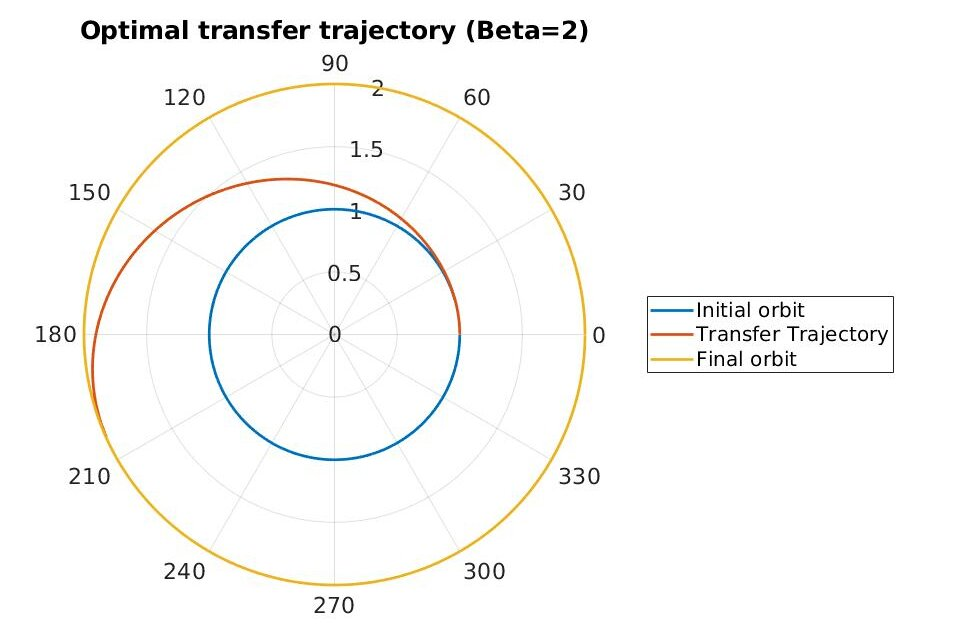
\includegraphics[width=\linewidth]{./jpgs/thrustArcB2.jpg}
    \caption{Numerically computed optimal transfer trajectory, $\beta = 2$.}
    \label{fig:Tarc-B2}
  \end{figure}


  \begin{figure}[H]
    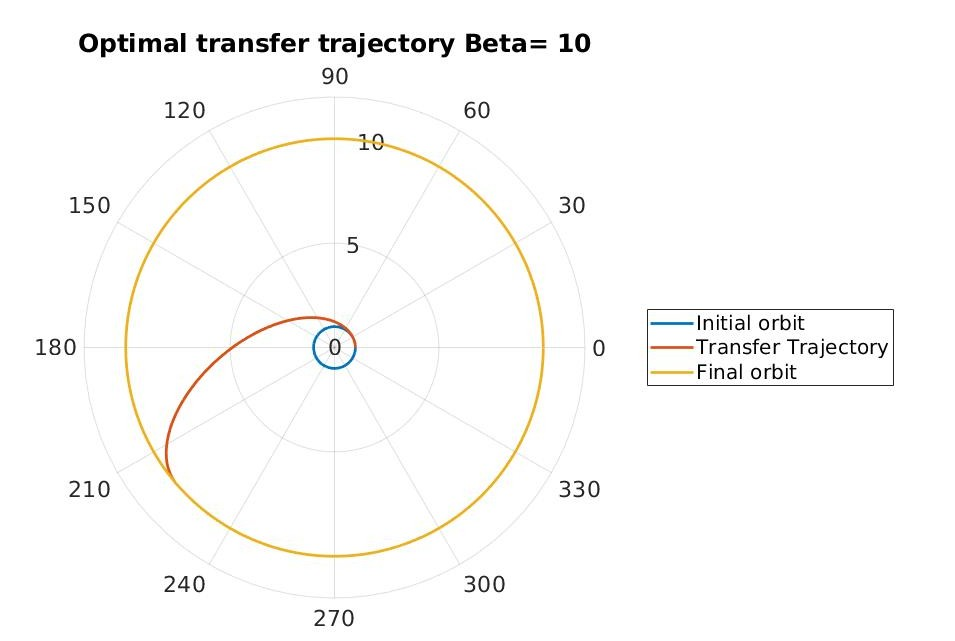
\includegraphics[width=\linewidth]{./jpgs/thrustArcB10.jpg}
    \caption{Numerically computed optimal transfer trajectory, $\beta = 10$.}
    \label{fig:Tarc-B10}
  \end{figure}



\begin{figure}[H]
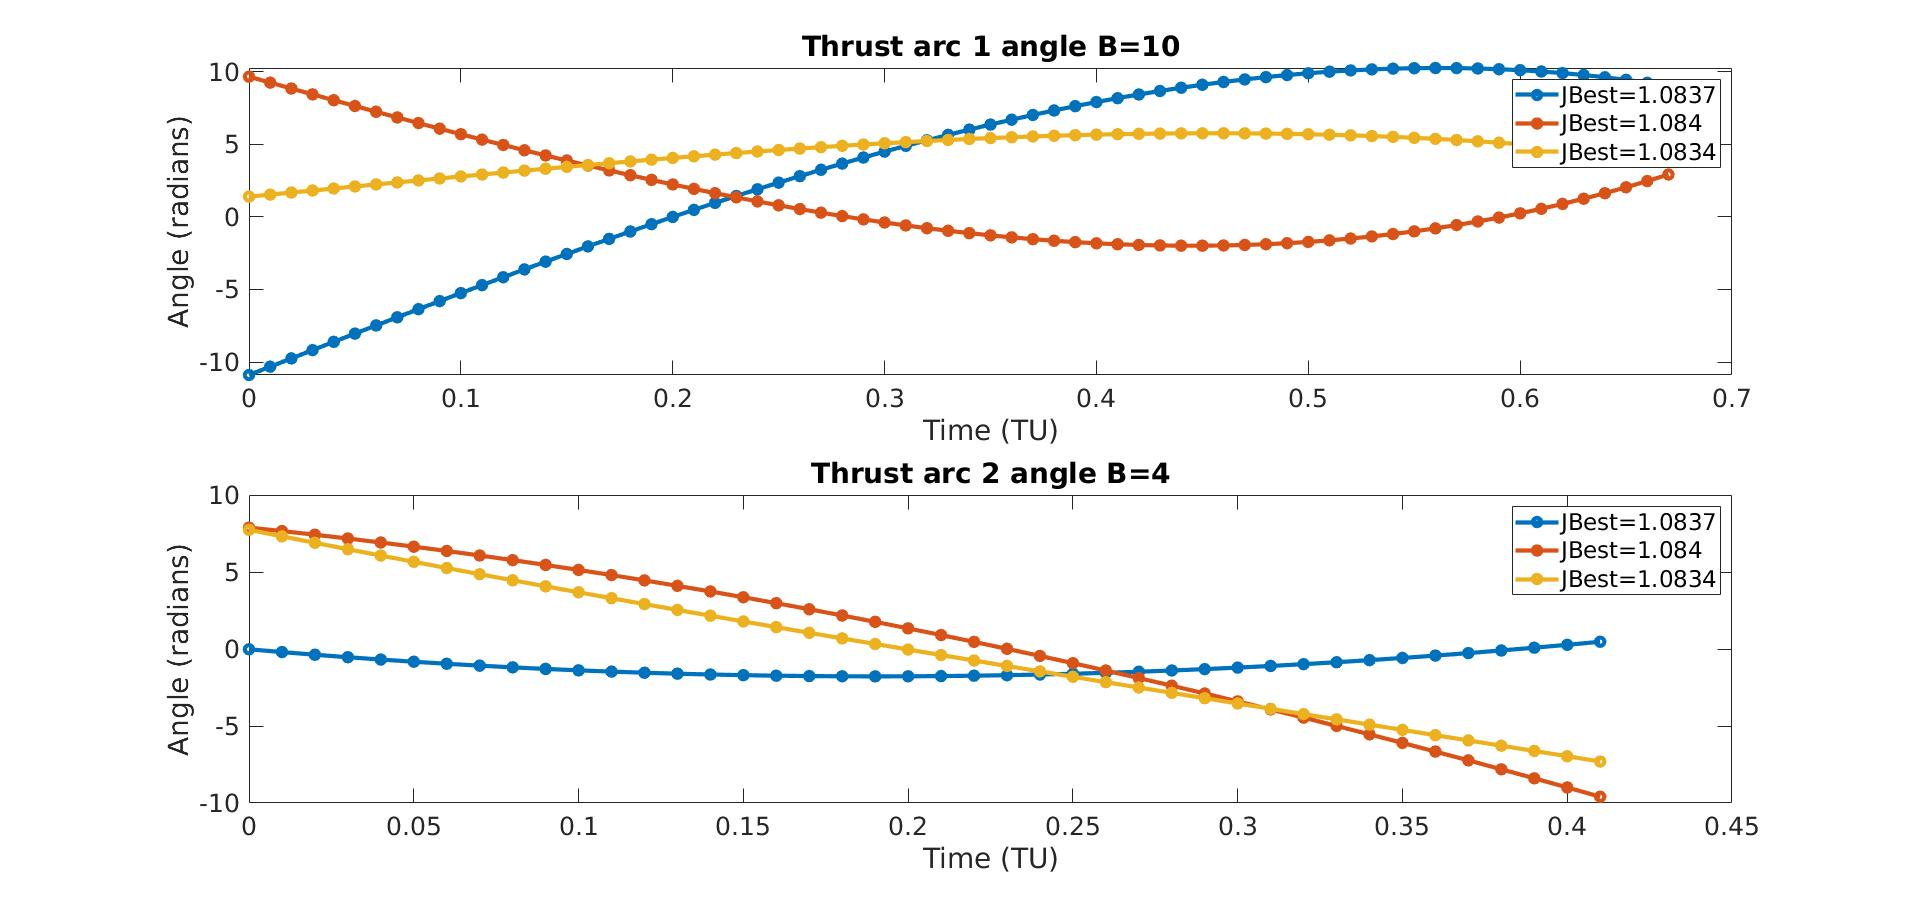
\includegraphics[width=\linewidth]{./jpgs/thrustAnglesB2.jpg}
\caption{Numerically computed thrust-angle time histories for optimal $\beta$ = 2 solutions  }
\label{fig:thrustAnglesB2}
\end{figure}

\begin{figure}[H]
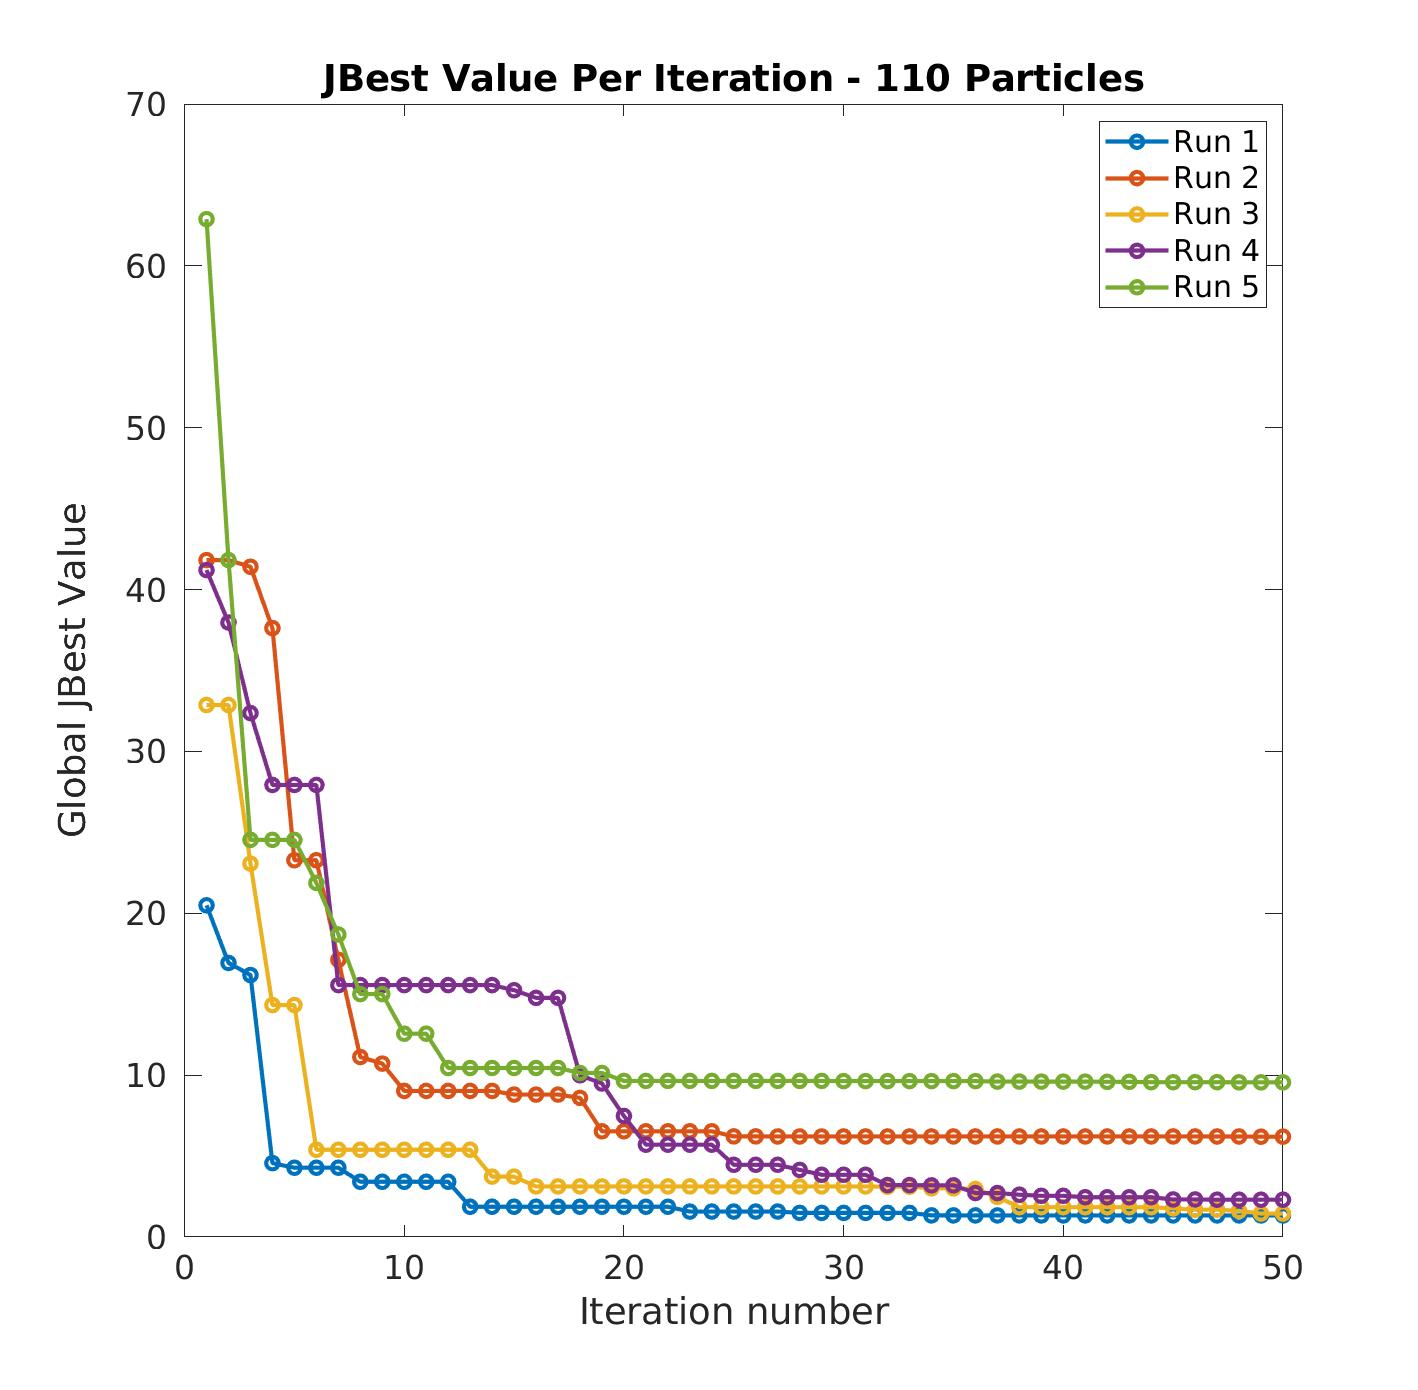
\includegraphics[width=\linewidth, height=13.5cm]{./jpgs/i50.jpg}
\caption{Global Best J Value Per Iteration: 100 Particles over 50 iterations}
\label{fig:gBestPer50Iter}
\end{figure}

\begin{figure}[H]
    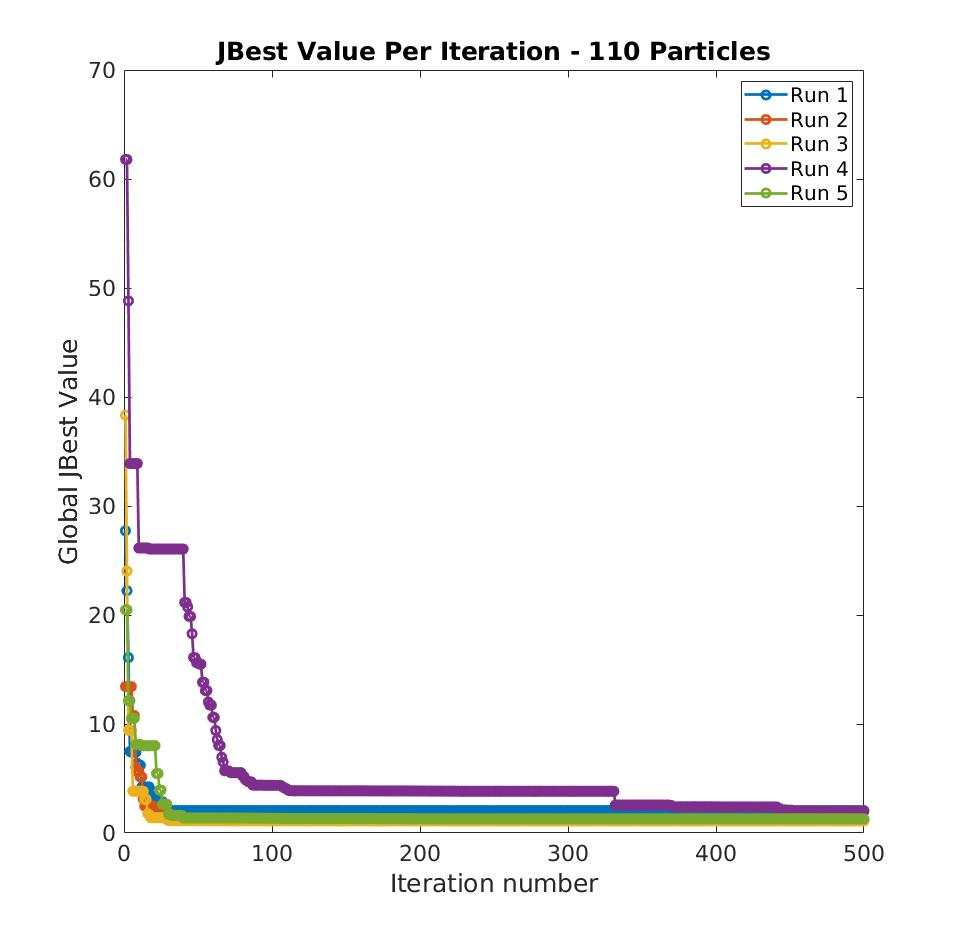
\includegraphics[width=\linewidth, height=13.5cm]{./jpgs/i500.jpg}
    \caption{Global Best J Value Per Iteration: 110 Particles over 500 iterations}
    \label{fig:gBestPer500Iter}
    \end{figure}
\section{Rehydration Results}

\begin{table}[H]
  \centering
  \begin{tabular}{lll|ll|ll}
    \toprule
    \multirow{2}{*}{25\% Rehydration} &
      \multicolumn{2}{c}{$\delta_{Javg}$ \textless .1\%} &
      \multicolumn{2}{c}{$\delta_{Javg}$ \textless 1\%} &
      \multicolumn{2}{c}{$\delta_{Javg}$ \textless 5\%} \\
      \cmidrule{2-7}
    & $\bar{J}_{best}$ & $\Delta \bar{J}_{best,\text{\%}}$ & $\bar{J}_{best}$ & $\Delta \bar{J}_{best,\text{\%}}$ & $\bar{J}_{best}$ & $\Delta \bar{J}_{best,\text{\%}}$ \\
    \midrule

    $n_{iter}=5$ & 1.347 & 44.177\% & 1.54 & 36.179\% & 1.438 & 40.406\% \\
    $n_{iter}=10$ & 1.421 & 41.11\% & 1.379 & 42.851\% & 1.594 & 33.941\% \\
    $n_{iter}=20$ & 1.331 & 44.840\% & 1.652 & 31.538\% & 1.503 & 37.712\% \\
    \bottomrule
  \end{tabular}
  \caption{Rehydration results for a 25\% population reset}
  \label{tab:rehydation-p25}
\end{table}

\begin{table}[H]
  \centering
  \begin{tabular}{lll|ll|ll}
    \toprule
    \multirow{2}{*}{33\% Rehydration} &
      \multicolumn{2}{c}{$\delta_{Javg}$ \textless .1\%} &
      \multicolumn{2}{c}{$\delta_{Javg}$ \textless 1\%} &
      \multicolumn{2}{c}{$\delta_{Javg}$ \textless 5\%} \\
      \cmidrule{2-7}
    & $\bar{J}_{best}$ & $\Delta \bar{J}_{best,\text{\%}}$ & $\bar{J}_{best}$ & $\Delta \bar{J}_{best,\text{\%}}$ & $\bar{J}_{best}$ & $\Delta \bar{J}_{best,\text{\%}}$ \\
    \midrule

    $n_{iter}=5$ & 1.371 & 43.18\% & 1.475 & 38.872\% & 1.412 & 41.484\% \\
    $n_{iter}=10$ & 1.364 & 43.47\% & 1.558 & 35.433\% & 1.473 & 40.448\% \\
    $n_{iter}=20$ & 1.412 & 41.48\% & 1.531 & 36.552\% & 1.578 & 34.604\% \\
    \bottomrule
  \end{tabular}
  \caption{Rehydration results for a 33\% population reset}
  \label{tab:rehydation-p33}
\end{table}


\begin{table}[H]
    \centering
    \begin{tabular}{lll|ll|ll}
      \toprule
      \multirow{2}{*}{50\% Rehydration} &
        \multicolumn{2}{c}{$\delta_{Javg}$ \textless .1\%} &
        \multicolumn{2}{c}{$\delta_{Javg}$ \textless 1\%} &
        \multicolumn{2}{c}{$\delta_{Javg}$ \textless 5\%} \\
        \cmidrule{2-7}
      & $\bar{J}_{best}$ & $\Delta \bar{J}_{best,\text{\%}}$ & $\bar{J}_{best}$ & $\Delta \bar{J}_{best,\text{\%}}$ & $\bar{J}_{best}$ & $\Delta \bar{J}_{best,\text{\%}}$ \\
      \midrule

      $n_{iter}=5$ & 1.58 & 34.52\% & 1.469 & 39.12\% & 1.425 & 40.94\% \\
      $n_{iter}=10$ & 1.396 & 42.15\% & 1.306 & 45.88\% & 1.473 & 38.96\% \\
      $n_{iter}=20$ & 1.373 & 43.10\% & 1.39 & 42.40\% & 1.33 & 44.88\% \\
      \bottomrule
    \end{tabular}
    \caption{Rehydration results for a 50\% population reset}
    \label{tab:rehydation-p50}
  \end{table}

\section{Speedup}

\subsection{MATLAB}

%Putting the H here ensures the table goes exactly where you put
%it in the code
\begin{table}[H]
    \centering
    \begin{tabular}{@{}llll@{}}
    \toprule
    \textbf{Num Particles} & \textbf{Num Iterations} & \textbf{Time (s)} \\ \midrule
    25                        & 250            & 30.527   \\
    25                        & 500            & 39.15    \\
    25                        & 1000           & 68.88    \\
    50                        & 250            & 30.527   \\
    50                        & 500            & 80.4246  \\
    50                        & 1000           & 141.151  \\
    100                      & 250            & 95.956   \\
    100                      & 500            & 152.22   \\
    100                      & 1000           & 306.732  \\
    150                      & 250            & 161.3    \\
    150                      & 500            & 195.87   \\
    150                      & 1000           & 388.03   \\
    200                      & 250            & 157.061  \\
    200                      & 500            & 251.575  \\
    200                      & 1000           & 457.55   \\ \bottomrule
    \end{tabular}
    \caption{MATLAB Numerical Results - Wall Clock Time}
    \label{tab:MATLAB-speedup}
    \end{table}

\subsection{C++ Single Threaded}

% Please add the following required packages to your document preamble:
% \usepackage{booktabs}
\begin{table}[H]
    \centering
    \begin{tabular}{@{}lllll@{}}
    \toprule
    \textbf{Num Particles} & \textbf{Num Iterations} & \textbf{Time (s)} & \bm{$n_{su\%}$} & \bm{$n_{su}$} \\ \midrule
    25          & 250  & 1.732    & 94.32633406          & 17.62528868              \\
    25          & 500 & 2.39     & 93.89527458          & 16.38075314              \\
    25          & 1000 & 3.92     & 94.30894309          & 17.57142857              \\
    50          & 250 & 2.96     & 90.30366561          & 10.31317568              \\
    50          & 500 & 3.26     & 95.94651388          & 24.6701227               \\
    50          & 1000 & 5.695    & 95.96531374          & 24.78507463              \\
    100         & 250 & 6.659    & 93.060361            & 14.40997147              \\
    100         & 500 & 7.21     & 95.2634345           & 21.11234397              \\
    100         & 1000 & 11.83    & 96.14321297          & 25.92831784              \\
    150         & 250 & 7.26     & 95.49907006          & 22.21763085              \\
    150         & 500 & 12.64    & 93.54674018          & 15.4960443               \\
    150         & 1000 & 16.68    & 95.7013633           & 23.26318945              \\
    200         & 250 & 7.77     & 95.05287754          & 20.21377091              \\
    200         & 500 & 11.423   & 95.45940574          & 22.02354898              \\
    200         & 1000 & 21.06    & 95.39722435          & 21.72602089              \\ \bottomrule
    \end{tabular}
    \caption{C++ Single Threaded Speedup Results - Wall Clock Time}
    \label{tab:ST-speedup}
    \end{table}


\subsection{C++ OpenMP}
\begin{table}[H]
    \centering
    \begin{tabular}{@{}llllll@{}}
    \toprule
    \textbf{Num Particles} & \textbf{Num Iterations} & \textbf{Time (s)} & \bm{$n_{su\%}$} & \bm{$n_{sust\%}$} & \bm{$n_{su}$} \\ \midrule
    25  & 250 & 1.78  & 94.16909621 & -2.771362587 & 17.15       \\
    25  & 500& 3.4   & 91.31545338 & -42.25941423 & 11.51470588 \\
    25  & 1000& 5.23  & 92.40708479 & -33.41836735 & 13.17017208 \\
    50  & 250 & 2.81  & 90.7950339  & 5.067567568  & 10.86370107 \\
    50  & 500& 4.77  & 94.06897889 & -46.3190184  & 16.86050314 \\
    50  & 1000& 8.51  & 93.9709956  & -49.42932397 & 16.58648649 \\
    100 & 250& 5.71  & 94.04935595 & 14.2513891   & 16.80490368 \\
    100 & 500& 6.6   & 95.66417028 & 8.460471567  & 23.06363636 \\
    100 & 100 & 11.73 & 96.17581472 & 0.8453085376 & 26.14936061 \\
    150 & 250 & 4.92  & 96.94978301 & 32.23140496  & 32.78455285 \\
    150 & 500 & 9.77  & 95.01199775 & 22.7056962   & 20.04810645 \\
    150 & 1000& 13.93 & 96.41007139 & 16.48681055  & 27.85570711 \\
    200 & 250 & 5.88  & 96.25623166 & 24.32432432  & 26.71105442 \\
    200 & 500 & 10.46 & 95.84219418 & 8.4303598    & 24.05114723 \\
    200 & 1000 & 22.42 & 95.09998907 & -6.457739791 & 20.40811775 \\ \bottomrule
    \end{tabular}
    \caption{OpenMP Speedup Results - Wall Clock Execution Time}
    \label{tab:OpenMP-speedup}
    \end{table}

\newpage
%%%%%%%%%%%%%%%%%%%%%%%%%%%%%%%%%%%%%%%%%%%%%%%%
% chapter5.tex                                 %
% Contains formatting and content of chapter 5 %
%%%%%%%%%%%%%%%%%%%%%%%%%%%%%%%%%%%%%%%%%%%%%%%%
\chapter{Conclusions and Recommendations for Future Work}

\section{Conclusions}
\noindent The finite thrust transfer problem models orbital transfers without
impulsive velocity change assumptions. As such, it provides higher fidelity
solutions for minimum propellant consumption maneuvers. An analysis of this problem
can direct thrust angles on a currently orbiting spacecraft throughout the transfer arc.
However, this algorithm requires significant time to confidently discover a quasi-optimal 
solution. In many cases, the necessity of determining optimal transfer parameters has minimal
advanced notice.
Thus, reducing the algorithm runtime and increasing the probability of optimal 
solution discovery is fundamental to enabling time-sensitive results. Significant improvements
in these bottlenecks could potentially enable on-board computers to calculate these transfer 
parameters autonomously. This thesis explores improvements to both of these barriers through algorithm 
benchmarking and a swarm stagnation prevention technique deemed \textit{rehydration}. \newline

\noindent While the particle swarm optimization algorithm runtime is inherently constrained by the 
calculations it entails, optimizing memory transfer, caching, and computation can potentially speed up its
execution. To explore this possibility, three different implementations of the algorithm were developed:
single threaded MATLAB, single threaded C++, and parallel C++. Each implementation ran for the $\beta = 2$
transfer over a range of $P_{num}$ and $I_{num}$ values. Results clearly indicated that C++ implementations 
are over an order of magnitude faster, peaking at a multiple of 26 times single threaded, and 32 times faster
parallelized. It can be observed that parallelizing the implementation improves efficiency throughout the
beginning portion of the algorithm, but has overhead outweighing the benefits during the exploitation phase of
particle swarm optimization. Toggling parallelization during program execution may allow for peak
efficiency throughout. The results from this benchmarking clearly demonstrate a significant improvement in 
algorithm performance. It is not unreasonable to consider real-time trajectory optimization maneuvers using 
similar C++ implementations in the future. \newline

\noindent The second problem this paper evaluates is increasing the probability of quasi-optimal solution 
discovery. As a stochastic algorithm, particle swarm optimization is prone to swarm stagnation, where the 
population prematurely converges on a non-optimal solution. \textit{Rehydration} is an attempt 
to rectify this behavior, resetting some of the population upon stagnation determination to inject more randomness
into the algorithm. \textit{Rehydration} results are tabulated for a series of the method's core parameters: $P_{r,\%}$,
$\delta_{Jcrit}$, $\eta_{iter}$, and compared against the average of 300 runs sans the reset technique. For each 
parameter combination, the \textit{rehydration} algorithm demonstrably improved the average solution discovered.
This indicates that this method can improve the probability of quasi-optimal solution discovery, thus reducing the 
amount of algorithm runs necessary to find optimal transfer parameters. In combination with C++ implementations, this significantly 
improves the two bottlenecks preventing real-time trajectory optimization.

\section{Recommendations For Future Work}

\noindent The core of this thesis proposes methods to improve the overall effectiveness of particle swarm 
optimization algorithms. While applied to the finite thrust transfer problem, their breadth is much further
reaching; these techniques can be used to optimize the solutions to a
wide variety of problems solved by computationally intensive particle swarm methods. Future work may be done in 
generalizing the C++ and \textit{rehydration} implementations and abstracting them for easy configuration and use 
in different problems. \newline

\noindent Additionally, this paper's exploration of concurrent programming as an algorithm optimization method
would benefit form a greater depth of research. As previously mentioned, developing an implementation with automatically
toggling parallelization based on swarm convergence state could help maintain peek efficiency throughout.
Other parallel implementations, namely graphical processing unit (GPU) programming, are also recommended to be considered. 
GPUs benefit from an immensely high thread count, enough for a thread per particle, but add increased overhead in copying
memory between host and device. An analysis of the tradeoffs between the increased multi-threaded efficiency and 
increased memory overhead is yet to be seen.

\newpage
% same for the backmatter
\backmatter
%%%%%%%%%%%%%%%%%%%%%%%%%%%%%%%%%%%%%%%%%%%%%%%%%%%%%%%%%%%%%%%%%%%%%%%%%%%%%%
% bibliography.tex                                                           %
% This file gives instructions for including and formatting the bibliography %
%%%%%%%%%%%%%%%%%%%%%%%%%%%%%%%%%%%%%%%%%%%%%%%%%%%%%%%%%%%%%%%%%%%%%%%%%%%%%%

\addcontentsline{toc}{chapter}{Reference} % adds the bibliography to the table of contents
\bibliography{backmatter/ugrad_thesis.bib} % this includes the bibliography
\bibliographystyle{unsrt} % change this to change the style of the bibliography and citations



\end{document}

